% Hotfix for issue with chngcntr:
\let\counterwithout\relax
\let\counterwithin\relax

% documentclass options:
\documentclass[11pt,
  a4paper,
  parskip=half, % This is some extra vertical space between paragraphs, the suggestion is 2cm which is really ugly, so we use what koma script gives us
  % you can also set it to full for even more space. But there is a bad tex style decision: parskip also changes the spacing between listitems such as
  % enumerate and itemize. For this purpose we include the enumitem package and set itemsep=.5em, of course you can change this
  BCOR=10mm, % BCOR is binding correction
  %ngerman,
  % if you'd rather have a one sided thesis, add `oneside' to the documentclass
  % oneside,
  % ngerman is needed for hyphenation if the thesis contains parts written in German, switch order with english if you write mainly in English.
  % Remember to change order in the babel package (below) as well.
  % Last language is the preferred one.
  english]{scrbook}
\usepackage[english]{babel} % If you write mainly in English change order to ngerman, english. Also change that in the documentclass options above.

% Other custom packages
\usepackage{amsmath}

% Include of titling must happen before \title etc.
% that's why it's not in setup.tex
\usepackage{titling}
\title{CurbNet: Semantic segmentation of curbs and curb cuts from street imagery}
\author{Yvan Putra Satyawan}

% Change to your first examiner
% The ~ enables non sentence spacing after a period
\newcommand{\firstexaminer}{Prof.~Dr.~Wolfram Burgard}
% Change to your second examiner, some undergraduate studies don't have a second examiner
% in this case just comment out the following line
\newcommand{\secondexaminer}{?}
% Change to your adivers
\newcommand{\advisers}{Jannik Zürn}

% include all packages and define commands in setup.tex

%------------------------------------------------------------------------------
%       package includes
%------------------------------------------------------------------------------
    % font encoding is set up for pdflatex, for other environments see
    % http://tex.stackexchange.com/questions/44694/fontenc-vs-inputenc
    \usepackage[T1]{fontenc}  % 8-bit fonts, improves handling of hyphenations
    \usepackage[utf8x]{inputenc}
    % provides `old' commands for table of contents. Eases the ability to switch
    % between book and scrbook
    \usepackage{scrhack}


    % ------------------- layout, default -------------------
    % adjust the style of float's captions, separated from text to improve readabilty
    \usepackage[labelfont=bf, labelsep=colon, format=hang, textfont=singlespacing]{caption}
    % With format = hang your caption will look like this:
    % Figure 1: Lorem ipsum dolor sit amet,
    %           consectetuer adipiscing elit.
    %           Ut purus elit, vestibulum
    % If you instead want
    % Figure 1: Lorem ipsum dolor sit amet,
    % consectetuer adipiscing elit. Ut purus
    % elit, vestibulum
    % change to format=plain
    \usepackage{chngcntr}  % continuous numbering of figures/tables over chapters
    \counterwithout{equation}{chapter}
    \counterwithout{figure}{chapter}
    \counterwithout{table}{chapter}

    % Uncomment the following line if you switch from scrbook to book
    % and comment the setkomafont line
    %\usepackage{titlesec}  % remove "Chapter" from the chapter title
    %\titleformat{\chapter}[hang]{\bfseries\huge}{\thechapter}{2pc}{\huge}
    \setkomafont{chapter}{\normalfont\bfseries\huge}

    \usepackage{setspace}  % Line spacing
    \onehalfspacing
    % \doublespacing  % uncomment for double spacing, e.g. for annotations in correction

    % ------------------- functional, default-------------------
    \usepackage[dvipsnames]{xcolor}  % more colors
    \usepackage{array}  % custom format per column in table - needed on the title page
    \usepackage{graphicx}  % include graphics
    \usepackage{subfig}  % divide figure, e.g. 1(a), 1(b)...
    \usepackage{amsmath}  % |
    \usepackage{amsthm}   % | math, bmatrix etc
    \usepackage{amsfonts} % |
    \usepackage{mathtools}
    \usepackage{calc}  % calculate within LaTeX
    \usepackage[unicode=true,bookmarks=true,bookmarksnumbered=true,
                bookmarksopen=true,bookmarksopenlevel=1,breaklinks=false,
                pdfborder={0 0 0},backref=false,colorlinks=false]{hyperref}
    \usepackage{etoolbox} % if-else commands


    %==========================================
    % You might not need the following packages, I only included them as they
    % are needed for the example floats
    % ------------------- functional, custom -------------------
    \usepackage[english, ruled]{algorithm2e}
    \usepackage{bm}  % bold greek variables (boldmath)
    \usepackage{tikz}
    \usetikzlibrary{positioning}  % use: above left of, etc
    
    % required for the ToDo list
    \usepackage{ifthen}

    % Improves general appearance of the text
    \usepackage[protrusion=true,expansion=true, kerning]{microtype}
    \usepackage{enumitem}
    % nicer font for pdf rendering
    %\usepackage{lmodern}
    
    % For nicer looking tables
    \usepackage{booktabs}

    % usually you don't need this, just for demonstration of a longer caption
    \usepackage{lipsum}

%------------------------------------------------------------------------------
%       (re)new commands / settings
%------------------------------------------------------------------------------
    % ----------------- referencing ----------------
    \newcommand{\secref}[1]{Section~\ref{#1}}
    \newcommand{\chapref}[1]{Chapter~\ref{#1}}
    \renewcommand{\eqref}[1]{Equation~(\ref{#1})}
    \newcommand{\figref}[1]{Figure~\ref{#1}}
    \newcommand{\tabref}[1]{Table~\ref{#1}}

    % ------------------- colors -------------------
    \definecolor{darkgreen}{rgb}{0.0, 0.5, 0.0}
    % Colors of the Albert Ludwigs University as in
    % https://www.zuv.uni-freiburg.de/service/cd/cd-manual/farbwelt
    \definecolor{UniBlue}{RGB}{0, 74, 153}
    \definecolor{UniRed}{RGB}{193, 0, 42}
    \definecolor{UniGrey}{RGB}{154, 155, 156}


    % ------------------- layout -------------------
    % prevents floating objects from being placed ahead of their section
    \let\mySection\section\renewcommand{\section}{\suppressfloats[t]\mySection}
    \let\mySubSection\subsection\renewcommand{\subsection}{\suppressfloats[t]\mySubSection}



    % ------------------- math formatting commands -------------------
    % define vectors to be bold instead of using an arrow
    \renewcommand{\vec}[1]{\mathbf{#1}}
    \newcommand{\mat}[1]{\mathbf{#1}}
    % tag equation with name
    \newcommand{\eqname}[1]{\tag*{#1}}


    % -------------- Table column formatting commands --------------
    \newcolumntype{L}{>{$}l<{$}}


    % ------------------- pdf settings -------------------
    % ADAPT THIS
    \hypersetup{pdftitle={\thetitle},
                pdfauthor={\theauthor},
                pdfsubject={Undergraduate thesis at the Albert Ludwig University of Freiburg},
                pdfkeywords={deep learning, convolutional neural networks,  undergraduate thesis, urban scene segmentation, scene segmentation},
                pdfpagelayout=OneColumn, pdfnewwindow=true, pdfstartview=XYZ, plainpages=false}


    %==========================================
    % You might not need the following commands, I only included them as they
    % are needed for the example floats

    % ------------------- Tikz styles -------------------
    \tikzset{>=latex}  % arrow style


    % ------------------- algorithm ---------------------
    % line spacing should be 1.5
    \renewcommand{\baselinestretch}{1.5}

    % set distance between items in a list, for more details see the
    % enumitem package: https://www.ctan.org/pkg/enumitem
    \setlist{itemsep=.5em}
    
    % use ra in your tables to increase the space between rows
    % 1.3 should be fine
    \newcommand{\ra}[1]{\renewcommand{\arraystretch}{#1}}

	% ToDo counters
	\usepackage{ifthen} %für whiledo-Schleife
	\newcounter{todos}
	\setcounter{todos}{0}
	\newcounter{extends}
	\setcounter{extends}{0}
	\newcounter{drafts}
	\setcounter{drafts}{0}

	% ------------------- marker commands -------------------
    % ToDo command
    \newcommand{\todo}[1]{\textbf{\textcolor{red}{(TODO: #1)}}\refstepcounter{todos}\label{todo \thetodos}}
	\newcommand{\extend}[1]{\textbf{\textcolor{darkgreen}{(EXTEND: #1)}}\refstepcounter{extends}\label{extend \theextends}}
	% Lighter color to note down quick drafts
	\newcommand{\draft}[1]{\textbf{\textcolor{NavyBlue}{(DRAFT: #1)}}\refstepcounter{drafts}\label{draft \thedrafts}}
	
	% microtype with lmodern, see https://tex.stackexchange.com/questions/75305/microtype-warning-with-lmodern-package-and-koma-script
	%\DeclareMicrotypeAlias{lmss}{cmr}

\begin{document}
    \pagestyle{empty} % no header and no page number
    % disable hyper links to remove warning "destination with same identifier"
    % this means within this section nothing can be referenced with a hyperlink
    \hypersetup{pageanchor=false}

    % enable/disable, depending on your chosen language
    
\begin{titlepage}
\begin{center}

\newcommand{\HorizontalLine}{\rule{\linewidth}{0.3mm}}

{\Large Undergraduate Thesis}\\[1.3cm]


% _____________________________________________________________________________
\HorizontalLine \\[0.4cm]
% Write your title in a fancy way like this if you want to customize it, otherwise simply let tex do it for you
% \begin{spacing}{3}
%     {\huge \bfseries The Long, Long } \\
%     {\huge \bfseries Long Long} \\
%     {\huge \bfseries Title}\\
% \end{spacing}
{ \huge \bfseries \thetitle }
\HorizontalLine \\[1.5cm]
% _____________________________________________________________________________


{\Huge \theauthor} \\[2cm]


\begin{tabular}[hc]{>{\huge}l >{\huge}l}
  Examiner: & \firstexaminer \\[0.3cm]
  Advisers: & \advisers \\[1.2cm]
\end{tabular}
\vfill  % move the following text to the bottom

\Large {
    Albert-Ludwigs-University Freiburg\\
    Faculty of Engineering\\
    Department of Computer Science\\
    Chair for Autonomous Intelligent systems\\[1cm]

    July 22\textsuperscript{nd}, 2019\\
}
\end{center}
\end{titlepage}

\thispagestyle{empty}
% title page back
\ \vfill \ \\  % at least one space required before vfill
\
\textbf{Writing Period}            \smallskip{} \\
04.\,20.\,2019 -- 07.\,22.\,2019   \bigskip{} \\
\
\textbf{Examiner}                  \smallskip{} \\
\firstexaminer                     \bigskip{} \\
\
% If there is a second examiner include it
\ifdef{\secondexaminer}
	{
	% Include
	\textbf{Second Examiner}       \smallskip{} \\
	\secondexaminer                \bigskip{} \\
	\
	}
	{
	% No second examiner, ignore
	}
\textbf{Advisers}                  \smallskip{} \\
\advisers

%    \pagestyle{plain} % remove chapter name from top, page number at the bottom
	\pagestyle{headings}
    % use \pagestyle{headings} for having the chapter on top of the pages
    % if you wang a more fancy header use \usepackage[automark,headsepline]{scrlayer-scrpage}
    % and read about it in the KOMA script documentation, https://www.ctan.org/pkg/koma-script
    \frontmatter  % roman page numbers
    % official declaration from the examination office; to be sure double
% check the wording on their website
% (https://www.tf.uni-freiburg.de/de/studium-lehre/a-bis-z-studium/dokumente/Declarationforthefinalthesis.pdf)

\chapter*{Declaration}

I hereby declare, that I am the sole author and composer of my thesis and that no other sources or learning aids, other than those listed, have been used.
Furthermore, I declare that I have acknowledged the work of others by providing detailed references of said work.  \newline
I also hereby declare, that my thesis has not been prepared for another examination or assignment, either in its entirety or excerpts thereof.
\\[3\normalbaselineskip]
\begin{tabular}{p{\textwidth/2} l}
  \rule{\textwidth/3}{0.4pt}   &   \rule{\textwidth/3}{0.4pt} \\
  Place, Date                  &   Signature
\end{tabular}

    \chapter*{Abstract}
In this work we propose CurbNet, a deep learning model based on DeepLab v3+ \cite{deeplab} with a modified version of cross entropy loss, for the purposes of curb and curb cut segmentation.
Using the encoder-decoder architecture from DeepLab v3+, CurbNet is capable of segmenting curbs and curb cuts in street-level imagery and can be used to aid the pathfinding pipeline used by the Obelix robot.
By adding this capability to Obelix, we can further its pathfinding capabilities \cite{europa}.
In this work, we show that CurbNet is a capable model, with its hyperparameters optimized using bayesian optimization and hyperband tuning \cite{bohb} and trained on the Mapillary dataset \cite{mapillary}.
    \chapter{Acknowledgments}

First and foremost, I would like to thank my parents Go Utama Handy Satyawan and Tuti Budiman for supporting me in my pursuit for a degree in Germany. Thank you for your support in giving me the opportunity to earn a Bachelor of Science in Computer Science.
I would also like to thank my advisor Jannik Zürn for the support and feedback he has given me during both the experimental and the writing phase of my thesis.
Thank you for helping me and being my guide in this journey through the sometimes opaque world of machine learning.

Huge thanks also to my friends Lukas König, Maximilian Roth, and Nina Pant for contributing ideas and their support throughout my time working on this thesis.

And finally, thank you to Prof. Dr. Wolfram Burgard for taking the time to look through my thesis and for any feedback you will provide.
    \tableofcontents
    \listoffigures
    \listoftables
    \hypersetup{pageanchor=true}  % re-enable hyperlinking

    \mainmatter  % Arabic page numbers
    \chapter{Introduction}\label{chap:introduction}
Semantic segmentation is a popular research topic in the field of computer vision, and particularly for autonomous vehicles.
The ability to semantically understand a scene is important for autonomous vehicles and robots to safely navigate an environment.
Generally, most implementations attempt to segment road surfaces but in this thesis, we propose the segmentation of curbs and curb cuts to allow safer sidewalk navigation.

The Europa project has resulted in the Obelix robotic platform, which has already been demoed to successfully perform pedestrian navigation~\cite{europa}\cite{obelix-slam}.
We propose to add to this platform the ability to detect curbs and curb cuts using semantic segmentation.
The Obelix platform is the result of a joint project to build a robotic platform capable of robotic navigation~\cite{europa}. 
In its current state, Obelix is already capable of localization and navigation using a map generated using LIDAR, but it is unable to determine what surface type it is driving on, e.g. asphalt, concrete, carpet, etc.~\cite{jannik}.
To extend its pathfinding ability, a project is currently underway to use the stereo cameras to classify surfaces that Obelix will encounter~\cite{jannik}.
This work specifically aims to add to said project by additionally identifying curbs and curb cuts, providing constraints for the route planner.
This will allow the route planner to identify curbs, which it cannot traverse, and curb cuts, which it can.

\begin{figure}
	\centering
	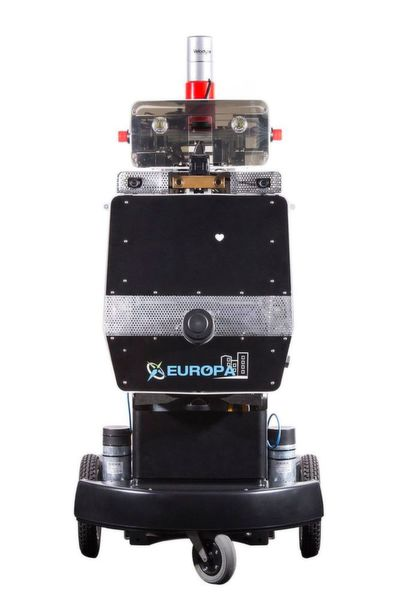
\includegraphics[width=.3\textwidth]{figures/introduction/obelix.jpg}
	\caption{The Obelix Robot platform developed by the Europa project. We plan to extend its path finding capabilities using the work in this thesis.}
\end{figure}

Our goal is thus to implement a computer vision algorithm capable of the semantic segmentation of curbs and curb cuts using a single camera image.
To do so, we implement a convolutional neural network (CNN) based on the paper "Encoder-Decoder with Atrous Separable Convolution for Semantic Image Segmentation" by Chen Liang Chieh et al~\cite{deeplab}.
We additionally include prior knowledge to the training, as it can be assumed that the camera setup and attitude for Obelix will remain relatively constant throughout its lifespan.

This thesis begins by discussing the motivation behind this thesis, followed by a discussion of related works and the background.
The approach is then discussed in detail along with the experiments and results.
Finally, a discussion of potential future research is be presented followed by the conclusion.

    \chapter{Related Work}\label{chap:relatedwork}
CurbNet uses semantic segmentation to identify curbs and curb cuts.
As such, related works can be divided into two categories: semantic segmentation and curb detection.
The following is a discussion of relevant related works.

\section{Image classification}\label{section:relatedwork-classification}
The field of semantic segmentation using trainable neural network models started in 1989 with the pioneering work of Eckhorn et al. and their paper describing how the visual cortex of a cat functions and its implications for network models~\cite{eckhorncat}.
This early method uses a pulse coupled neural network, which produces synchronous bursts of pulses, effectively grouping the neurons by phase and pulse frequency, which can then be analyzed for feature extraction.

In the same year, Y. LeCun et al. developed the first algorithm to use backpropagation and convolutional neural networks to identify and classify images~\cite{zipcode}.
Their paper titled "Backpropagation Applied to Handwritten Zip Code Recognition" proposes using convolutional filters directly on an image input and training using backpropagation.
This technique is able to reliably classify images into predetermined classes.
This is the first network architecture that took a normalized image as input and returned the image class directly as an output.
LeCun et al. also shows that using backpropagation to learn the convolutional filter coefficients performed significantly better than using hand selected coefficients.
This pioneering work set the stage for modern day image classification and segmentation algorithms using CNNs and automated learning.

"Very Deep Convolutional Networks for Large-Scale Image Recognition" by Karen Simonyan and Andrew Zisserman and published in 2014 is one of the earlier works to show that a deeper network setup could result in very high accuracy image classification~\cite{vgg}.
Their setup improves upon the use of convolutional neural networks by proposing instead to use small $\left(3 \times 3\right)$ convolutional filters and changing the depth to 16-19 layers.
This network is now commonly known as VGG16 - VGG19, with the number corresponding to layer depth.
This simple change in architectural design results in their architecture securing first and second place in the ImageNet Challenge 2014 localization and classification tracks respectively~\cite{vgg}.
The authors do note that these very deep networks tended to overfit on smaller datasets and were difficult to train.

"Deep Residual Learning for Image Recognition" by Kaiming He et al. and published in 2016 proposes a solution to this problem~\cite{resnet}.
They reformulate the layers as learning residual functions and use the layer inputs as references.
This architecture is now commonly known as ResNet.
By doing so, they are able to empirically show that their residual networks are easier to optimize and have lower complexity despite being up to eight times deeper than VGG networks.
ResNet was able to obtain a 28\% relative improvement on the COCO object detection dataset compared to previous methods~\cite{coco}.

\section{Semantic Segmentation}\label{section:relatedwork-segmentation}
"Fully Convolutional Networks for Semantic Segmentation" by Jonathan Long et al. and published in 2015 takes these classification networks and added fully convolutional layers to take the encoded features and use it for semantic segmentation~\cite{fcn}.
This paper lays out a novel insight to the problem of image segmentation as nothing more than a dense image classification problem.
The proposed network architecture is now commonly referred to as FCN.
In essence, they propose that image segmentation is nothing more than image classification on a per-pixel basis.
As such, previously developed CNNs for image classification could be used as a feature encoder for semantic segmentation networks.
They show that their network, using VGG16 as its feature encoder, was able to outperform competing state-of-the-art approaches on the PASCAL Visual Object Challenge dataset by a relative margin of 20\% \cite{pascal}.

DeepLab v3+, proposed in "Encoder-Decoder with Atrous Separable Convolution for Semantic Image Segmentation" by Liang-Chieh Chen et al. improves on FCN by refining the segmentation, especially along object boundaries~\cite{deeplab}.
DeepLab v3+ became the basis of the network we used for CurbNet.
Using pyramid pooling and an improved encoder-decoder architecture, DeepLab v3+ achieves 89.0\% mean intersection over union (IoU) accuracy on the Cityscapes dataset~\cite{cityscapes}.

\section{Curb Detection}\label{section:relatedwork-curbdetection}
"Curb Detection for a Pedestrian Robot in Urban Environments" by Jérôme Maye, Ralf Kaestner, and Roland Siegwart, published in 2012, uses the LIDAR sensors that Obelix has to map the world around it \cite{ethobelix}.
Using this point cloud data, a virtual representation of the environment can be computed and horizontal planes from the scene extracted.
By detecting sudden changes in the vertical position of horizontal planes, a curb can be implicitly identified.
This relies on the assumption that curbs take the form of vertical planes connecting two horizontal planes.
This work does not take into account curb cuts, which may not necessarily form a significant vertical height difference and are usually sloped.

"WalkNet: A Deep Learning Approach to Improving Sidewalk Quality and Accessibility" by Andrew Abbott et al. and published in 2018 specifically addresses the identification of curb cuts~\cite{walknet}.
This paper proposes the use of a deep neural network to classify images in which curb cuts existed.
Their goal is the use of Google Street View data to map which intersections in a city have curb cuts and which do not.
This data is then to be supplied to city governments to provide relevant information regarding sidewalk accessibility and quality.
This work is focussed on the classification images which contained curb cuts and not the segmentation of said curb cuts. The neural network architecture they used was not described in depth.
    \chapter{Background}\label{chap:background}
Explain the math and notation.
\begin{algorithm}[p]
\caption{Stochastic Gradient Descent: Neural Network}
\label{alg:backpropnn}
\begin{algorithmic}
    % \ttfamily
    \State Create a mini batch of $m$ samples $\vec{x}_0 \ldots \vec{x}_{m-1}$
    \ForEach{sample $\vec{x}$}
        \State $\vec{a}^{\vec{x},0} \gets \vec{x}$  \alignedComment{Set input activation}
        \ForEach{Layer $l \in \{1\ldots L-1\}$}  \alignedComment{Forward pass }
            \State $\vec{z}^{\vec{x},l} \gets \mathbf{W}^l \vec{a}^{\vec{x},l-1}+\vec{b}^l$
            \State $\vec{a}^{\vec{x},l} \gets \varphi(\vec{z}^{\vec{x},l})$
        \EndFor
        \State $\bm{\delta}^{\vec{x},L} \gets \nabla_{\vec{a}} C_\vec{x} \odot \varphi'(\vec{z}^{\vec{x},L})$ \alignedComment{Compute error}
        \ForEach{Layer $l \in L-1, L-2 \ldots 2$}  \alignedComment{Backpropagate error}
            \State $\bm{\delta}^{\vec{x},l} \gets ((\mathbf{W}^{l+1})^T \bm{\delta}^{\vec{x},l+1})\odot \varphi'(\vec{z}^{\vec{x},l})$
        \EndFor
    \EndFor
    \ForEach{$l \in L, L-1 \ldots 2$} \Comment  \alignedComment{Gradient descent}
        \State $ \mathbf{W}^l \gets \mathbf{W}^l-\frac{\eta}{m} \sum_\vec{x} \bm{\delta}^{\vec{x},l} (\vec{a}^{\vec{x},l-1})^T$
        \State $\vec{b}^l \gets \vec{b}^l-\frac{\eta}{m}\sum_\vec{x} \bm{\delta}^{\vec{x},l}$  
    \EndFor
\end{algorithmic}
\end{algorithm}


\begin{figure}[t]
    \begin{center}
    \begin{tikzpicture}
        \node (a) at (0,0) {a};
        \node (b) at (2, 0) {b};
        \draw[->] (a) -- (b);
        

    \end{tikzpicture}
    \end{center}
    \caption[Tikz Example]{Use tikz to draw nice graphs!}
    \label{fig:Tikz}
\end{figure}
    \chapter{Approach}\label{chap:approach}
To semantically segment urban scenes and extract predictions for curbs and curb cuts, we proposed to use a deep neural network based on the DeepLab v3+ architecture with a loss function inspired by "U-Net: Convolutional Networks for Biomedical Image Segmentation" by Olaf Ronneberger et al. \cite{unet}.
In this chapter, the architecture used and an explanation of our loss function will be discussed.

\section{Architecture Selection} \label{section:approach-architectureselection}
Relative to the entire image, curb and curb cut classes make up a relatively small proportion of the image, making up 0.986\% and 0.196\% of images on average respectively.
As such, four networks with good known performance for urban scene segmentation were chosen and evaluated for their performance classifying curbs and curb cuts.
We experimented with ENet, described in the paper "ENet: A Deep Neural Network Architecture for Real-Time Semantic Segmentation" \cite{enet}; GoogLeNet ,described in the paper "Going Deeper with Convolutions" \cite{googlenet}; FCN16s, described in "Fully Convolutional Networks for Semantic Segmentation" \cite{fcn}; and DeepLab v3+, described in the paper "Encoder-Decoder with Atrous Separable Convolution for Semantic Image Segmentation" \cite{deeplab}.
To evaluate which network would have the most potential, we trained each network on a small subset of the whole dataset to find which networks would converge the fastest given a certain budget.
This was done to compare how each network would perform classifying curbs and curb cuts.

We came to use the DeepLab v3+ architecture after running these experiments due to significantly outperforming the other networks, as seen in \todo{make table}.

\subsection{Modifications to DeepLab v3+}\label{section:approach-extendingdeeplab}
Given that we are working with the assumption of a camera with a constant attitude, we can also make the assumption that curbs will be more likely towards the bottom and sides of an image.
Therefore, we modified DeepLab v3+ by adding a preprocessing step which turns the input image into a five-dimensional tensor, with the fourth and fith dimensions being the x and y coordinates of the pixel, respectively.
The initial convolutional layer was also modified to accept five channels as input.
\extend{add image of example tensor input showing what each channel is}

\subsection{Network Architecture}\label{section:approach-networkarchitecture}
We propose to apply the DeepLab v3+ architecture to our stated problem of curb and curb cut classification with the modifications described in subsection \ref{section:approach-extendingdeeplab}.
The architecture itself is described in Table \ref

\begin{table}
	\begin{tabular}{|c|c|}
		content...
	\end{tabular}
\end{table}

\section{Loss Function}\label{section:approach-lossfunction}
Initially, the network was trained on standard cross entropy loss, but due to the severe class imbalance, this did not produce meaningful results with the network simply labeling everything as the 0th class, i.e. not curb or curb cut.
We then used a weighted cross entropy loss function.
The weights were chosen by taking the normalized inverse of the average proportion other, curb, and curb cut classes in the dataset.
This provided better results, but was still not producing the results that we wanted \todo{make this sound more formal and include image}.

Using the assumption that all curbs and curb cuts must be located along the perimeter of roads, we used a loss function inspired by the paper "U-Net: Convolutional Networks for Biomedical Image Segmentation" which we call Masked Cross Entropy (MCE) and can be seen in \eqref{eq:mce} \cite{unet}.
The weighted cross entropy loss function was modified to penalize according to the given weights when labeling within a certain border around road classes, which we call the mask $M$.
We define road classes $\text{class}_{\text{road}}$ as all classes which can reasonably be expected to be found on roads, including road, road markings, potholes, etc.
This mask was calculated using a binary dilation on a full $b \times b$ matrix $B$ where $b$ is $0.03 \times \text{image}_{width}$ on the road class, then subtracted by the road class itself.
Thus, this can be formalized as follows:
\begin{align}
	B &= \underbrace{
			\begin{bmatrix}
				1  & \cdots & 1\\ 
				\vdots &  \ddots & \vdots\\ 
				1 &  \cdots & 1
				\end{bmatrix}}_{b \text{ columns and } b \text{ rows}} \\
	M &= \left(\text{class}_{\text{road}} \oplus B\right) - \text{class}_{\text{road}}
\end{align}

The value 0.03 was chosen by the researcher after looking at samples in the dataset and measuring what area around roads are typically curbs.
The road class was simply taken from the ground truth data.
Any labeling outside of $M$ by the network are then given an increased penalty, incentivizing the network to focus labeling around road edges.
We chose to multiply the penalty for areas outside $M$ by a factor of 3.
This can be seen in the following formalization of the loss function we used:
\begin{align}\label{eq:mce}
	\text{loss}_{MCE}(x, class) &= weight[class]\left(-\log\left(\frac{\text{exp}(x[class])}{\sum_{j}\text{exp}(x[j])}\right)\right)\\
	\text{with } weight[class] &= 
	\begin{cases}
	weight'[class] & \text{if} x \in M\\
	weight'[class] \cdot 3 & \text{if} x \notin M
	\end{cases}
\end{align}
where $weight'[class]$ are the user defined weights. 
This loss function operates on the assumption that curbs and curb cuts must be located adjacent to roads.
A visualization of the resulting mask $M$ can be seen in \todo{image of mask}.

    \chapter{Experiments}\label{chap:experiments}
A series of experiments were carried out to determine the performance of the network in its stated goal of classifying curbs and curb cuts. To this end, the network was tested on the Mapillary Vistas dataset \cite{mapillary} and its hyperparameters optimized using the Bayesian optimization with hyperband (BOHB) procedure from the AutoML group at the University of Freiburg \cite{bohb}

\section{Dataset} \label{section:experiments-dataset}
The Mapillary Vistas dataset was chosen for this task as it was, to our knowledge, the only street-level dataset that included ground truth segmentations of both curbs and curb cuts.
This dataset contains images from all around the world and includes images captured from different imaging devices including mobile phones, action cameras, and professional imaging solutions.
These images are captured during various weather, seasonal, and daylight conditions.
As such, the dataset provides a challenging level of diversity.

With such a diverse dataset, the images must first be preprocessed.
We process all the images to conform to a 4:3 size ratio, eliminate images without images of curbs or curb cuts, and extract only road, curb, and curb cut classes.

To optimize training speed with respect to wall clock time, and given the computational constraints, images were resized for training.
The chosen image resolution was $360 \times 320$ pixels. 
This allows a batch size of 16 per GPU, given that the GPU has 12 GB of VRAM.
To further optimize training, the images are resized prior to training and the resized images stored.
This allows all training and validation images to be loaded into memory, reducing the number of file accesses required and reducing training wall clock time by a factor of two.

After running an analysis of the dataset with respect to their curb and curb cut content and image dimensions, we found that there were 15,160 usable images in the training set and 1610 usable images in the validation set.
Usable images in this case refers to images that contains both curbs and curb cuts.
A detailed results of the analysis of can be found in Appendix section \ref{appendix:dataset}.

\section{Network Evaluation}\label{section:experiments-networkevaluation}
Experiments were done to evaluate the performance of different networks on our dataset.
Specifically, we identified the small size of curbs relative to the rest of the image causes a severe class imbalance and increases the difficulty in recognizing the smaller features.

Relative to the entire image, curb and curb cut classes make up a relatively small proportion of the image, making up 0.986\% and 0.196\% of images on average respectively.
As such, three networks with good known performance for urban scene segmentation were chosen and evaluated for their performance classifying curbs and curb cuts.
We experimented with GoogLeNet, described in the paper "Going Deeper with Convolutions"~\cite{googlenet}; FCN16s, described in "Fully Convolutional Networks for Semantic Segmentation"~\cite{fcn}; and DeepLab v3+, described in the paper "Encoder-Decoder with Atrous Separable Convolution for Semantic Image Segmentation"~\cite{deeplab}.

To evaluate which network would have the most potential, we trained each network on a small subset of the whole dataset to find which networks would converge the fastest given a certain budget.
For each of these runs, the default recommended hyperparameters were used due to time constraints to conduct hyper-parameter optimization with every network.
The results can be seen in \figref{chart:experiments-networkcomparison} and in \tabref{tab:network-comparison}.
Given these results, we chose to use DeepLab v3+ as our network.

% Please add the following required packages to your document preamble:
% \usepackage{booktabs}
% \usepackage{graphicx}
\begin{table}[b]
	\centering
	\begin{tabular}{@{}ll@{}}
		\toprule
		Network     & mIoU \\ \midrule
		DeepLab v3+ & 30.83\%   \\
		FCN16s      & 19.97\%   \\
		GoogLeNet   & 25.08\%   \\ \bottomrule
	\end{tabular}
	\caption[Network Comparison Results]{Results of running the DeepLab v3+, FCN16s, and GoogLeNet on a subset of the main dataset after one thousand iterations. It can be seen that DeepLab v3+ was able to achieve the highest mIoU performance overall.}
	\label{tab:network-comparison}
\end{table}
\begin{figure}
	\centering
	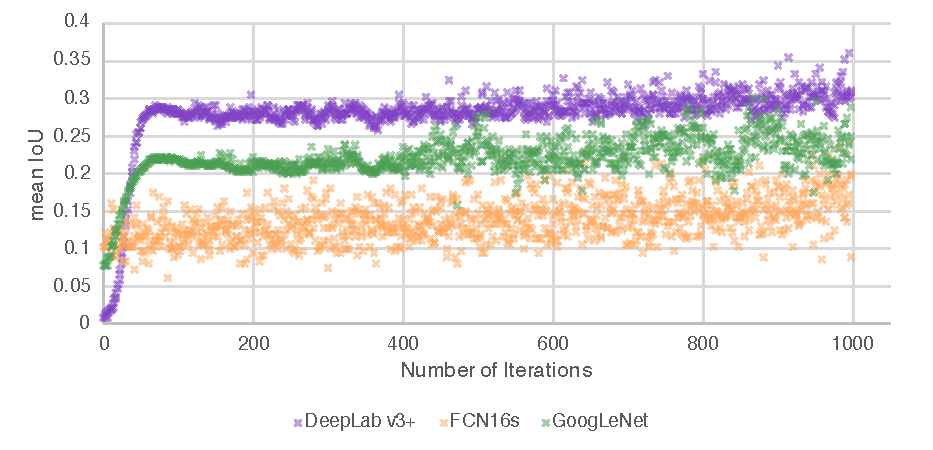
\includegraphics[width=\textwidth]{figures/experiments/network-comparison.pdf}
		\caption[Network Comparison Chart]{Training mIoU Accuracy over 1000 Iterations using DeepLab v3+, FCN16s, and GoogLeNet. It can be seen that DeepLab v3+ achieves the best mIoU performance overall.}
		\label{chart:experiments-networkcomparison}
\end{figure}

\section{Modifications to DeepLab v3+}\label{section:experiments-modifications}
Given that we are working with the assumption of a camera with a constant attitude, we can also make the assumption that curbs will be more likely towards the bottom and sides of an image.
Therefore, modifications were made to DeepLab v3+ by adding a preprocessing step which turns the input image into a five-dimensional tensor, with the fourth and fifth dimensions being the $x$ and $y$ coordinates of the pixel, respectively.
The initial convolutional layer was also modified to accept five channels as input.
Both versions of the network were run with identical hyperparameters on a limited budget and dataset.
While there was an increase in mean IoU accuracy when using the five-dimensional input tensor, it was negligible and we decided to use the three-dimensional input tensor, given the increased training time with a five-dimensional input tensor.

\todo{include 5D vs 3D results}

\section{Loss Function Evaluation}\label{section:experiments-loss}
Our custom loss function masked cross entropy loss was evaluated against weighted cross entropy loss.
The results, shown in \figref{chart:experiments-losstraining} and \ref{chart:experiments-lossvalidation}.
These results show that the validation loss was similar for the first 2370 iterations.
After this point, masked cross entropy loss shows a clear advantage in validation accuracy compared to weighted cross entropy loss.
After 4740 iterations, shows a clear performance advantage, with a difference of 5.56 mean IoU percentage points.
As such, we have chosen to implement our network using masked cross entropy loss as our loss function.

\begin{figure}
	\centering
	\begin{subfigure}{\textwidth}
		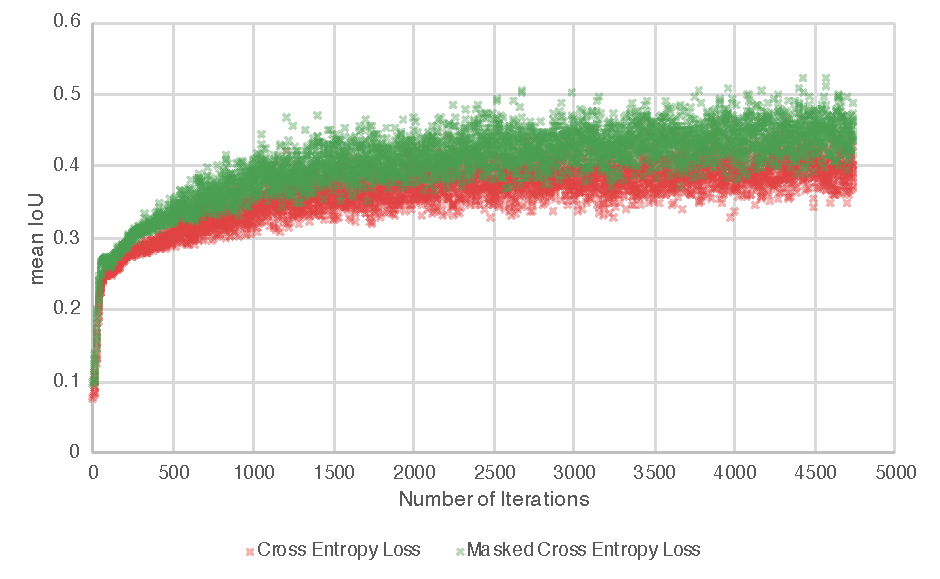
\includegraphics[width=\textwidth]{figures/experiments/loss-comparison-training.pdf}
		\caption[Loss Comparison Chart: Training]{Training mIoU Accuracy over 4740 Iterations comparing weighted cross entropy loss and masked cross entropy loss. The results show that although performing similarly to begin with, masked cross entropy loss was able to outperform weighted cross entropy loss.}
		\label{chart:experiments-losstraining}
	\end{subfigure}
	\newline
	\begin{subfigure}{\textwidth}
		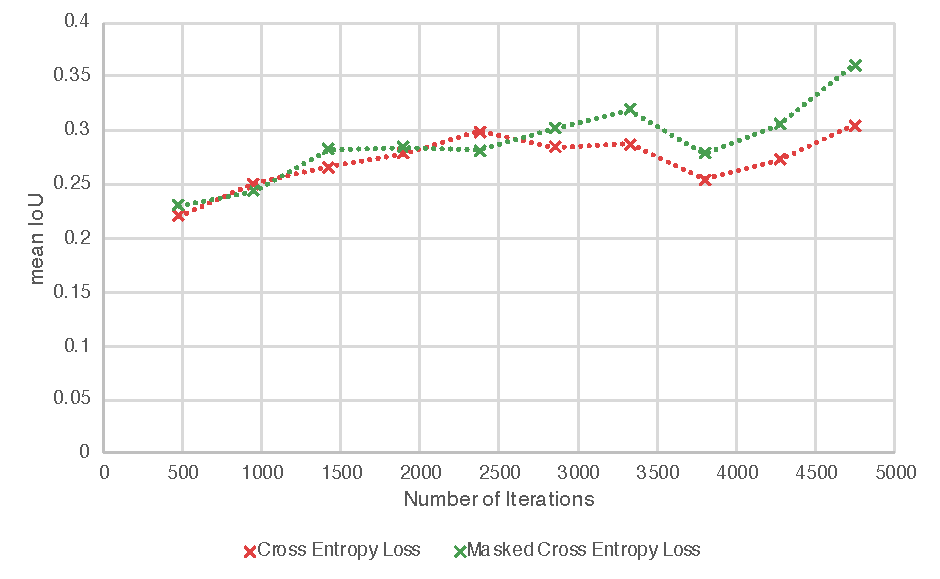
\includegraphics[width=\textwidth]{figures/experiments/loss-comparison-validation.pdf}
		\caption[Loss Comparison Chart: Validation]{Validation mean IoU Accuracy over 4740 Iterations, measured every 474 iterations, comparing cross entropy loss and masked cross entropy loss. Validation accuracy was evaluated against a validation set of 1680 images. The lines shown in the chart are to emphasize the data.}
		\label{chart:experiments-lossvalidation}
	\end{subfigure}
	\caption[Loss Comparison Chart]{Comparisons of masked cross entropy loss and weighted cross entropy loss. Both loss functions were evaluated using the same hyperparameters against a dataset consisting of 15160 training images and 1680 validation images.}
\end{figure}

\section{Hyperparameters} \label{section:experiments-hyperparameters}
Hyperparameter tuning was done by using Bayesian Optimization with HyperBand.
The hyperparameters that were tuned were the learning rate; optimizer; momentum, if the optimizer chosen was stochastic gradient descent; epsilon, if the optimizer chosen was Adam; the weight ratio for the loss weights; and the loss criterion.

The learning rate is optimized between the interval $\left[1 \times 10^{-5}, 1 \times 10^{-2}\right]$, varied on a logarithmic scale.
The optimizer is a categorical choice between stochastic gradient descent or Adam.
The momentum is optimized between the interval $\left[0, 0.99\right]$.
The epsilon value is optimized between the interval $\left[1 \times 10^{-2}, 1\right]$.
The weight ratio for the loss weight determines the ratio of the weights between the curb and curb cut.
The value of the weight for the "other" class is one-tenth of the sum of curb and curb cut weights, formally defined as:
\begin{equation}
	\begin{split}
		\frac{x}{y} &= r, ~r \in \left[2, 6\right]\\
		z &= \frac{x + y}{10}
	\end{split}
\end{equation}
where $x$ is the weight for the curb class, $y$ the weight for the curb cut class, $z$ the weight for the "other" class, and $r$ the ratio value that is optimized.
The loss criterion is a categorical choice between weighted cross entropy loss or masked cross entropy loss.
Further details of the hyperparameters optimized can be found in \tabref{tab:hyperparameters}.
\todo{make sure cross entropy loss or masked cross entropy loss}
% Please add the following required packages to your document preamble:
% \usepackage{booktabs}
\begin{table}[]
\begin{tabular}{@{}llp{3.9cm}p{3cm}@{}}
\toprule
Parameter Name    & Parameter Type & Range                                            & Comments                               \\ \midrule
Learning rate     & Float          & $\left[1 \times 10^{-5}, 1 \times 10^{-2}\right]$& On a logarithmic scale                \\
Optimizer         & Categorical    & Adam or SGD                                      &                                      \\
SGD momentum      & Float          & $\left[0, 0.99\right]$                           & Only active when the optimizer is SGD\\
Adam epsilon      & Float          & $\left[1 \times 10^{-2}, 1\right]$               & Only active when the optimizer is Adam\\
Loss weight ratio & Float          & $\left[2,6\right]$                               &                                       \\
Loss criterion    & Categorical    & Weighted cross entropy or masked cross entropy   &                                      \\ \bottomrule
\end{tabular}
\caption[Hyperparameter Details]{Table of hyperparameters and their values that were optimized for using Bayesian Optimization and HyperBand.}
\label{tab:hyperparameters}
\end{table}

\extend{include graph}
The hyperparameters are optimized according to the above parameters using a cluster of \todo{number of} GPUs over a budget of 12 iterations.
The resulting optimized values for the hyperparameters are in \tabref{tab:hyperparameterresults}.
More detailed results of each run of the hyperparameter optimization can be found in Appendix section \ref{appendix:hpoptimresults}.

Given increased compute resources and time, we believe that we could further optimize the hyperparameters and achieve better results with our network.

% Please add the following required packages to your document preamble:
% \usepackage{booktabs}
\begin{table}[]
	\centering
\begin{tabular}{@{}lp{2.3cm}}
\toprule
Parameter Name    & Value     \\ \midrule
Learning rate     & 0.0002    \\
Optimizer         & Adam      \\
SGD momentum      & -         \\
Adam epsilon      & 0.1       \\
Loss weight ratio & 4         \\
Loss criterion    & Masked cross entropy loss\\ \bottomrule
\end{tabular}
\caption[Hyperparameter Optimization Results]{Table of hyperparameters and their values that were optimized for using Bayesian Optimization and HyperBand. \todo{complete table values}}
\label{tab:hyperparameterresults}
\end{table}

\section{Training Pipeline} \label{section:experiments-trainingpipeline}
The training pipeline is a main script which calls the training loop with a set of parameters defined in either a JSON file or through command-line arguments.
Using a JSON file makes it simpler to change parameters as nothing is hard-coded and command-line arguments do not have to be memorized or meticulously typed out each time.

A Graphical User Interface (GUI) is also available, made using the tkinter framework, which is capable of visualizing the ground truth segmentation, the network output, a live display of the current loss and mean IoU accuracy, and other statistics.
This GUI can be seen in \figref{fig:experiments-gui}.

A Command Line Interface (CLI) is also available, made using the ncurses framework, which is capable of displaying various statistics during training.
The CLI also allows training remotely using secure shell (SSH), as the GUI would fail to start if invoked remotely through the command line.
A screen capture of the CLI can be seen in \figref{fig:experiments-cli}

\begin{figure}
	\centering
	\begin{subfigure}{0.45\textwidth}
		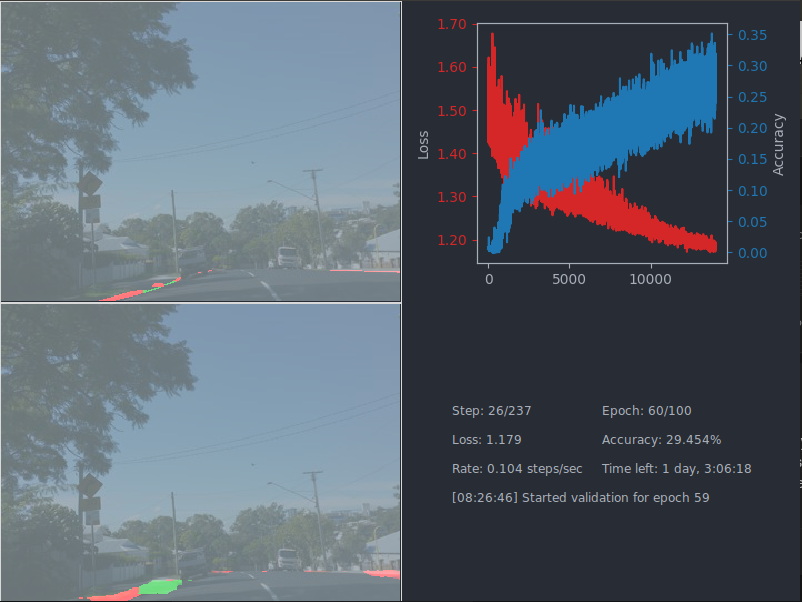
\includegraphics[width=\linewidth]{figures/experiments/gui.png}
		\caption[Training GUI]{A screen capture of the GUI that was used to visualize training results. In clockwise from the top left, the GUI visualizes the ground truth data, a live plot of the loss and accuracy, various statistics, and the network output.}
		\label{fig:experiments-gui}
	\end{subfigure}
	\hfill
	\begin{subfigure}{0.45\textwidth}
		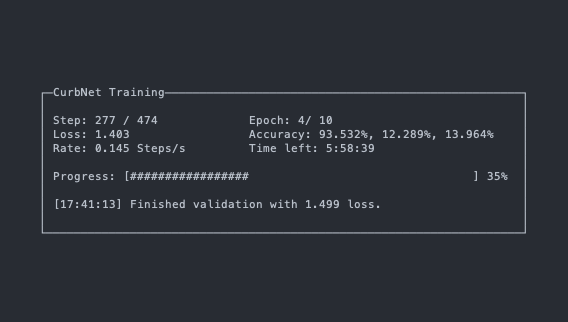
\includegraphics[width=\linewidth]{figures/experiments/cli.png}
		\caption[Training CLI]{A screen capture of the CLI that was used to train the network remotely.}
		\label{fig:experiments-cli}
	\end{subfigure}
	\caption[Training UI]{The two available user interfaces available to use with CurbNet. The GUI was mean to more simply and quickly deliver the most important information first to the researcher. The CLI was designed to allow training status along with the most pertinent information to be shown remotely with little overhead.}
\end{figure}

The different components necessary to train the network are written in such a way as to be modular, with nearly everything being easily configurable.
For example, the network, optimizer, and loss criterion can easily be swapped by changing command-line arguments or parameters in the JSON file.
This makes running different experiments straightforward.

\section{Evaluation Metrics} \label{section:experiments-evaluationmetrics}
The mean Intersection over Union (mIoU) is the main evaluation metric chosen.
IoU measures the intersection of the prediction and the ground truth data, divided by the union of the prediction and the ground truth data.
This is done on a per class basis and then averaged to get the mIoU.


\section{Results}\label{section:experiments-results}
Running our network with the optimal hyperparameters chosen by the hyperparameter search in Section \ref{section:experiments-hyperparameters} for \todo{how many iterations did we train} iterations, we were able to achieve an accuracy of \todo{value}.
We were able to train the network for \todo{how many before overfit} before the network started overfitting to the training set.

The network is able to produce the segmentations seen in \todo{include figure}.

Analyzing these results, we can see that the network excels at \todo{what does it excel at}.
Surprisingly, the network can even identify curbs and curb cuts which are in the distance and thus have a relatively small size.
In these cases, the segmentation is significantly larger than the size of the curb itself, i.e. even though the intersection is significant, there is a significant area around the curb that is falsely identified as part of the curb.
An example of this can be seen in \todo{figure}

The main failure modes of the network are falsely identifying non-curb road edges as curbs and identifying certain road markings as curbs.
Certain road edges which have a different texture, but are not raised, are sometimes also segmented as curbs.
Certain road markings which are located near road edges are also sometimes segmented as curbs.
Examples of both of these cases can be seen in figure \todo{figure}
We hypothesize that this may be a result of the network not having depth information.

Given depth information, it may be possible to reduce these false positives and further increase the performance of the network.

    \chapter{Future Research}\label{chap:future-research}
    \chapter{Conclusion}\label{chap:conclusion}
    % Input any files for appendix here
\chapter{Appendix}
% This will include the results of the hyperparameter optimization
\section{Detailed Hyperparameter Optimization Results}\label{appendix:hpoptimresults}

\begin{table}[h!]
	\centering
	\begin{tabular}{@{}clllll@{}}
		\toprule
		& \multicolumn{5}{c}{Parameter} \\\cmidrule(lr){2-6}
		Run Number & Learning rate & Optimizer & Momentum & Epsilon & Loss criterion \\ \midrule
		1 & $2.017 \times 10^{-5}$ & Adam & - & 0.8 & MCE \\
		2 & $3.567 \times 10^{-5}$ & Adam & - & 0.95 & MCE \\
		3 & $8.073 \times 10^{-5}$ & Adam & - & 0.4 & MCE \\
		4 & $2.116 \times 10^{-5}$ & SGD & 0.5 & - & MCE \\ \bottomrule
	\end{tabular}
	\caption[Hyperparameter Tuning Configurations]{Hyperparameter configurations used for each run performed. These were the values selected by the bayesian optimization and hyperband algorithm used to optimized the hyperparameters for the CurbNet model.}
	\label{tab:appendix-hpoptimconfig}
\end{table}

% Please add the following required packages to your document preamble:
% \usepackage{booktabs}
\begin{table}[h!]
	\centering
	\begin{tabular}{@{}crrrr@{}}
		\cmidrule(r){1-4}
		& \multicolumn{3}{c}{IoU} &  \\ \cmidrule(lr){2-4}
		Run Number & Curb & Curb Cut & Ignore & mIoU \\ \midrule
		1 & 0.918\% & 0.125\% & 50.919\% & 17.320\% \\
		2 & 0.860\% & 0.136\% & 51.222\% & 17.406\% \\
		3 & 0.080\% & 22.450\% & 83.008\% & 35.179\% \\
		4 & 0.414\% & 0.289\% & 68.653\% & 23.11\% \\ \bottomrule
	\end{tabular}
	\caption[Hyperparameter Tuning Results]{Hyperparameter tuning results based on the configurations in Table \ref{tab:appendix-hpoptimconfig} after performing bayesian optimization and hyperband tuning with a budget of 5-10 epochs for each configuration.}
	\label{tab:appendix-hpoptimresults}
\end{table}
\newpage
\section{Dataset Statistics}\label{appendix:dataset}

% Please add the following required packages to your document preamble:
% \usepackage{booktabs}
\begin{table}[h!]
	\centering
	\begin{tabular}{@{}p{0.7\textwidth}l@{}}
		\toprule
		Statistic & Value\\ \midrule
		Total images & 18,000 \\
		Maximum image dimensions & $\left(6528 \times 5248\right)$ \\
		Minimum image dimensions & $\left(640 \times 480\right)$ \\
		Number of different dimensions & 156 \\
		Percent of images with curbs & 84.21667\% \\
		Percent of images with curb cuts & 44.79444\% \\
		Average proportion of image that are curbs & 0.81557\% \\
		Average proportion of images that contain curbs that are curbs & 0.96842\% \\
		Average proportion of image that are curb cuts & 0.08869\% \\
		Average proportion of images that contain curb cuts that are curb cuts & 0.19799\% \\
		Images with curb cuts but without curbs & 30 \\ 
		Usable Images (contains both curbs and curb cuts) & 15160 \\\bottomrule
	\end{tabular}
	\caption{General dataset statistics}
	\label{tab:appendix-dataset}
\end{table}


    
    % If you want a list of your ToDos at the end of the document
    % don't forget to remove before submission!
    % place it somewhere in the document
\chapter*{ToDo Counters}
\newcounter{ct}%
To Dos: \arabic{todos}; \hspace{1em}%
\setcounter{ct}{0}%
\whiledo {\value{ct} < \value{todos}}%
{%
	\stepcounter {ct}%
    \ref{todo \thect}%
	\ifnum\value{ct} = \value{todos}{}\else{, }\fi
}

Parts to extend: \arabic{extends}; \hspace{1em}%
\setcounter{ct}{0}%
\whiledo {\value{ct} < \value{extends}}%
{%
	\stepcounter {ct}%
	\ref{extend \thect}%
	\ifnum\value{ct} = \value{extends}{}\else{, }\fi
}

Draft parts: \arabic{drafts}; \hspace{1em}%
\setcounter{ct}{0}%
\whiledo {\value{ct} < \value{drafts}}%
{%
	\stepcounter {ct}%
	\ref{draft \thect}%
	\ifnum\value{ct} = \value{drafts}{}\else{, }\fi
}


    \bibliographystyle{ieeetr}
    \bibliography{bib/topic1}
    % bibliography is not in the table of contents per default, add it manually
    \addcontentsline{toc}{chapter}{Bibliography}
    \todo{replace all arXiv links with journal links, if possible}
    \newpage
    \thispagestyle{empty}
    \mbox{}


\end{document}
